% Class Notes Template
\documentclass[12pt]{article}
\usepackage[margin=1in]{geometry} 
\usepackage[utf8]{inputenc}

% Packages
\usepackage[french, english]{babel}
\usepackage{amsmath, amsthm, amssymb ,amsfonts, graphics, tikz, float, enumerate, graphicx}
\usepackage{listings, booktabs}
\usepackage{color} %red, green, blue, yellow, cyan, magenta, black, white
\definecolor{mygreen}{RGB}{28,172,0} % color values Red, Green, Blue
\definecolor{mylilas}{RGB}{170,55,241}

\lstset{language=Matlab,%
	%basicstyle=\color{red},
	breaklines=true,%
	morekeywords={matlab2tikz},
	keywordstyle=\color{blue},%
	morekeywords=[2]{1}, keywordstyle=[2]{\color{black}},
	identifierstyle=\color{black},%
	stringstyle=\color{mylilas},
	commentstyle=\color{mygreen},%
	showstringspaces=false,%without this there will be a symbol in the places where there is a space
	numbers=left,%
	numberstyle={\tiny \color{black}},% size of the numbers
	numbersep=9pt, % this defines how far the numbers are from the text
	emph=[1]{for,end,break},emphstyle=[1]\color{blue}, %some words to emphasise
	%emph=[2]{word1,word2}, emphstyle=[2]{style},    
}

% Title
\title{ECON 6140 - Problem Set \# 3}
\date{\today}
\author{Julien Manuel Neves}

% Use these for theorems, lemmas, proofs, etc.
\newtheorem{theorem}{Theorem}
\newtheorem{corollary}[theorem]{Corollary}
\newtheorem{lemma}[theorem]{Lemma}
\newtheorem{observation}[theorem]{Observation}
\newtheorem{proposition}[theorem]{Proposition}
\newtheorem{definition}[theorem]{Definition}
\newtheorem{claim}[theorem]{Claim}
\newtheorem{fact}[theorem]{Fact}
\newtheorem{assumption}[theorem]{Assumption}
\newtheorem{problem}[theorem]{Problem}
\newtheorem{set-up}[theorem]{Set-up}
\newtheorem{example}[theorem]{Example}
\newtheorem{remark}[theorem]{Remark}
\newtheorem{axiom}[theorem]{Axiom}

% Usefuls Macros
\newcommand{\field}[1]{\mathbb{#1}}
\newcommand{\N}{\field{N}} % natural numbers
\newcommand{\R}{\field{R}} % real numbers
\newcommand{\Z}{\field{Z}} % integers
\newcommand\F{\mathcal{F}}
\newcommand\B{\mathbb{B}}
\renewcommand{\Re}{\R} % reals
\newcommand{\Rn}[1]{\mathbb{R}^{#1}}
\newcommand{\1}{{\bf 1}} % vector of all 1's
\newcommand{\I}[1]{\mathbb{I}_{\left\{#1\right\}}} % indicator function
\newcommand{\La}{\mathscr{L}}
% \newcommand{\tends}{{\rightarrow}} % arrow for limits
% \newcommand{\ra}{{\rightarrow}} % abbreviation for right arrow
% \newcommand{\subjectto}{\mbox{\rm subject to}} % subject to

%% math operators
\DeclareMathOperator*{\argmin}{arg\,min}
\DeclareMathOperator*{\argmax}{arg\,max}
\DeclareMathOperator*{\maximize}{maximize}
\DeclareMathOperator*{\minimize}{minimize}
\DeclareMathOperator{\E}{\mathsf{E}} % expectation
\newcommand{\Ex}[1]{\E\left\{#1\right\}} % expectation with brackets
\DeclareMathOperator{\pr}{\mathsf{P}} % probability
\newcommand{\prob}[1]{\pr\left\{#1\right\}}
\DeclareMathOperator{\subjectto}{{s.t.\ }} % subject to
\newcommand{\norm}[1]{\left\|#1\right\|}
\newcommand{\card}[1]{\left|#1\right|}

% Extra stuff
\newcommand\seq[1]{\{ #1 \}}
\newcommand{\inp}[2]{\langle #1, #2 \rangle}

\newcommand{\inv}{^{-1}}

\newcommand{\pa}[1]{\left(#1\right)}
\newcommand{\bra}[1]{\left[#1\right]}
\newcommand{\cbra}[1]{\left\{ #1 \right\}}

\newcommand{\pfrac}[2]{\pa{\frac{#1}{#2}}}
\newcommand{\bfrac}[2]{\bra{\frac{#1}{#2}}}

\newcommand{\mat}[1]{\begin{matrix}#1\end{matrix}}
\newcommand{\pmat}[1]{\pa{\mat{#1}}}
\newcommand{\bmat}[1]{\bra{\mat{#1}}}

\begin{document}

\maketitle

Buckle up! This problem set as a lot of code and very few comments in it.  I would have loved to make it neater, but I ran out of time and .

\section*{Problem \#1}


\begin{enumerate}[(a)]
\item


See \texttt{main.m}, \texttt{tauchen.m}, and \texttt{transition.m}. Moreover, see Tab~\ref{tab:tab1}. Note that $\Ex{y_t}=e^{\mu+\frac{\sigma^2}{2}}$ where $\mu$ and $\sigma^2$ are the expected moments of $w_t$. Hence, for $\Ex{y_t}=1$ ,we need
\[
\bar{w}=-(1-\rho)\frac{\sigma_\epsilon^2}{2(1-\rho^2)}
\]


\item

See \texttt{main.m}, \texttt{tauchen.m}, \texttt{rouwenhorst.m}, and \texttt{transition.m}. The results are reported in Tab~\ref{tab:tab1}. It seems that the Tauchen method does fairly well to approximate $\rho$ and $\sigma_\epsilon$. Note that increasing the number of states seems to have a ambiguous effectiveness. My guess is that with an even number of states, we are indirectly missing the point with the highest probability mass, i.e. $\mu$. Hence, $9$ states could potential do better than only $5$ states or even $10$ states.

\begin{table}[H]
	\centering
	\label{tab:tab1}
	\begin{tabular}{@{}lll@{}}
		\toprule
		& $\rho$   & $\sigma_{\epsilon}$ \\ \midrule
		Model               & $.90$     & $.24495$            \\
		Tauchen (5 points)  & $.92665$ & $.26813$            \\
		Tauchen (10 points) & $.89168$ & $.27535$            \\ \bottomrule
	\end{tabular}
	\caption{Tauchen with 5 points and 10 points}
\end{table}

\item
See \texttt{main.m}, \texttt{tauchen.m}, \texttt{rouwenhorst.m}, and \texttt{transition.m}. The results are reported in Tab~\ref{tab:tab2}. Clearly, the Rouwenhorst is yields the best approximation of $\rho$ and $\sigma_\epsilon$ since it perfectly matches the parameters.
\begin{table}[H]
	\centering
	\label{tab:tab2}
	\begin{tabular}{@{}lll@{}}
		\toprule
		& $\rho$   & $\sigma_{\epsilon}$ \\ \midrule
		Model               & $.90$     & $.24495$            \\
		Tauchen (5 points)  & $.92665$ & $.26813$            \\
		Rouwenhorst (5 points) & $.90$ & $.24495$            \\ \bottomrule
	\end{tabular}
	\caption{Tauchen with 5 points and Rouwenhorst 5 points}
\end{table}

\item
See \texttt{main.m}, \texttt{tauchen.m}, \texttt{rouwenhorst.m}, and \texttt{transition.m}. The results are reported in Tab~\ref{tab:tab3}. Lo, and behold! Even with $\rho$ close to $0$, the Rouwenhorst perfectly matches $\rho$ and $\sigma_\epsilon$.

\begin{table}[H]
	\centering
	\label{tab:tab3}
	\begin{tabular}{@{}lll@{}}
		\toprule
		& $\rho$   & $\sigma_{\epsilon}$ \\ \midrule
		Model               & $.98$     & $.012505$            \\
		Rouwenhorst (5 points) & $.98$ & $.012505$            \\ \bottomrule
	\end{tabular}
	\caption{Rouwenhorst 5 points and high $\rho$}
\end{table}

 Note that to match $var(w_t)$, we need to decrease $\sigma_\epsilon$. In fact, we need
\[
\sigma_\epsilon^2 = \frac{\sigma_{\epsilon,old}^2(1-\rho^2)}{(1-\rho^2_{old})}
\]

\end{enumerate}
\section*{Problem \#2}

\begin{enumerate}[(a)]
	\item
	
	I modified Prof. Huckfedlt's code to get rid of the pesky globals and try to reduce everything to functions. See \texttt{main.m}, \texttt{policy\_ip.m}, \texttt{euler\_ip.m}, and \texttt{solve\_ip.m}. Fig~\ref{fig:fig1} and Fig~\ref{fig:fig2} chose the decision rules for consumption and $a'(a,y)$ respectively. 
		\begin{figure}[H]
		\centering
		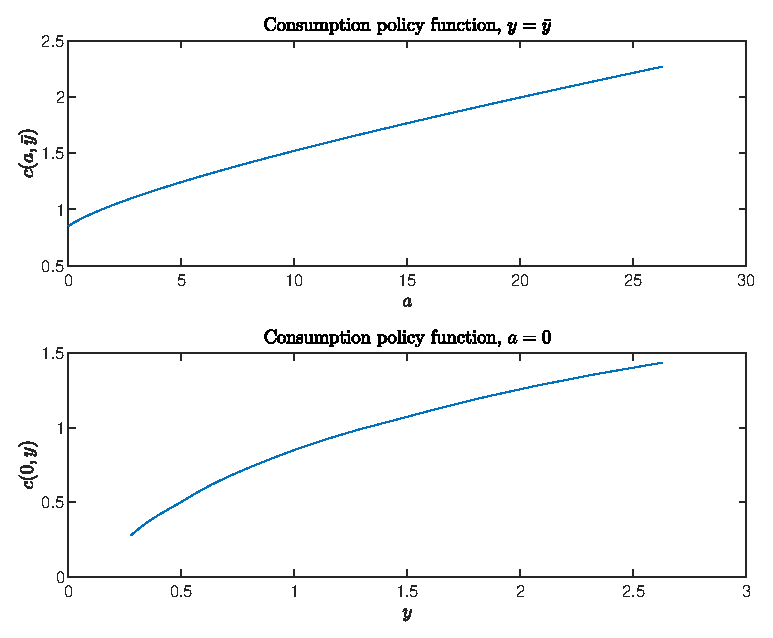
\includegraphics[width=0.7\linewidth]{fig1}
		\label{fig:fig1}
		\caption{Consumption policy function}
	\end{figure}
Note that for low $y$ and $a=0$, the borrowing constraints binds and we get the bent shape in our savings policy function. 

	\begin{figure}[H]
		\centering
		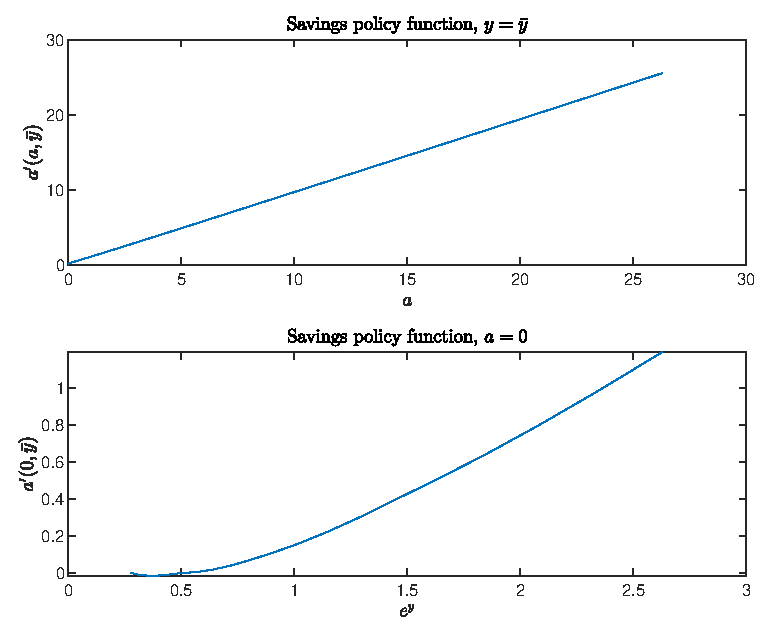
\includegraphics[width=0.7\linewidth]{fig2}
		\label{fig:fig2}
				\caption{Savings policy function}
	\end{figure}
\item



See \texttt{markovchain.m}, and \texttt{markovprob.m} for the Markov chain simulation. The results for the unconditional standard deviation of $c$ are reported in Tab~\ref{tab:tab4}.
\begin{table}[H]
	\centering
	\label{tab:tab4}
	\begin{tabular}{@{}llc@{}}
		\toprule
		& &$\sigma_c$    \\ \midrule
		$\gamma = 1$      &          & $.49118	$               \\
		$\gamma = 2$  &             & $.44302$              \\
		$\gamma = 5$ & & $.39500$            \\ \bottomrule
	\end{tabular}
	\caption{$\sigma_c$ for different values of $\gamma$}
\end{table}




\item

Fig~\ref{fig:fig3} plots the saving rates given $a=0$ for different $y$. 
	\begin{figure}[H]
	\centering
	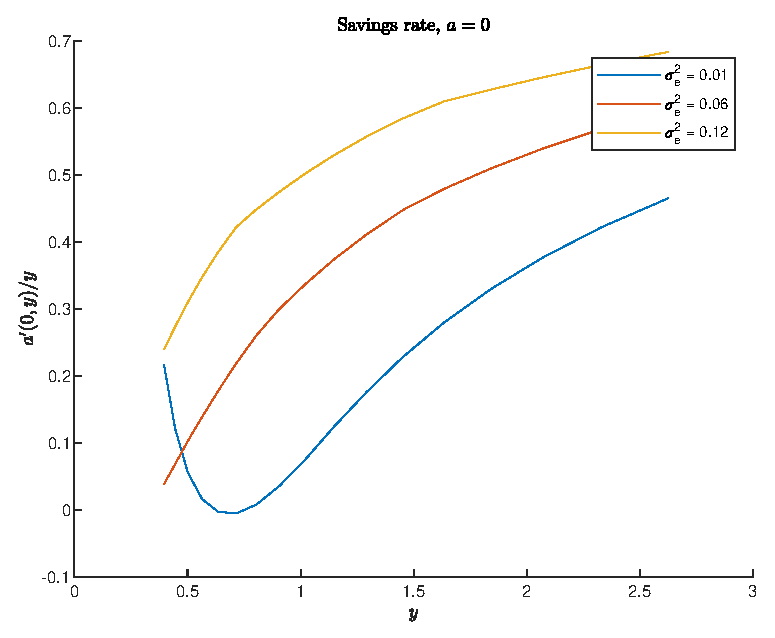
\includegraphics[width=0.7\linewidth]{fig3}
	\label{fig:fig3}
	\caption{Savings rate}
\end{figure}

Note that as $\sigma_\epsilon$ increases, the savings rate also increases for all possible $y$. Hence, $\sigma_\epsilon$ increasing, implies higher volatility in income and therefore higher motive for precautionary savings. Please disregard the left part of the curve for $\sigma_\epsilon^2=0.01$. This is result is simply a consequence of how our grid was set up.

\item

The results for the mean $c$ with different borrowing constraints are reported in Tab~\ref{tab:tab5}.
\begin{table}[H]
	\centering
	\label{tab:tab5}
	\begin{tabular}{@{}llc@{}}
		\toprule
		& &$\bar{c}$    \\ \midrule
		$a\geq0$      &          & $1.0571	$               \\
		$a\geq-\frac{y_{min}}{r}$  &             & $.92897$        \\ \bottomrule
	\end{tabular}
	\caption{$\bar{c}$ for different borrowing constraints}
\end{table}

It seems that having a looser borrowing constraint, implies lower average consumption. This is the results of having less motive for precautionary savings. Hence, by saving less, people get less consumption later on. While the value of utility might be higher due to the timing of consumption with the natural borrowing constraint, we get still get that on average consumption is lower than with no-borrowing.

\item

The results for the insurance coefficient with different borrowing constraints are reported in Tab~6.
\begin{table}[H]
	\centering
	\label{tab:tab6}
	\begin{tabular}{@{}llc@{}}
		\toprule
		& &$\psi$    \\ \midrule
		$a\geq0$      &          & $.56445	$               \\
		$a\geq-\frac{y_{min}}{r}$  &             & $.57244$        \\ \bottomrule
	\end{tabular}
	\caption{$\psi$ for different borrowing constraints}
\end{table}
Note that having a looser borrowing constraint, implies higher insurance coefficient. In fact, if $\epsilon_t$ and $c_t$ are more correlated, then shocks to income will directly transfer to shocks to consumption. This in turns will decrease $\psi$, since the $c_t$ are not protected against income volatility. Hence, natural borrowing constraint with its higher $\psi$ implies that people are not a scared of shocks that could reduce their income since they are basically never restricted in their borrowing unlike $a\geq0$.


\end{enumerate}


\section*{Problem \#3}


\begin{enumerate}[(a)]
	\item
	
	Let $x_t = (1+r_t)a_t+y_{t}$ or $x=Ra+y$. Then,
	\begin{align*}
		c+a'\leq Ra+y\\
		c+\frac{x'-y'}{R}\leq x\\
		Rc+{x'-y'}\leq Rx\\
		x'\leq R(x-c)+y'
	\end{align*}
	and
	\begin{align*}
	a'\geq 0\\
	\frac{x'-y'}{R}\geq 0\\
	{x'}\geq y'\\
	x\geq c
	\end{align*}
	
	Now, since our process is i.i.d., we have $\pi(y',y) = \pi(y')$. Hence, in this problem, $y$ is not a state variable, but it does influence the expected value of $x'$ since it is a function $y'$. Thus, our cash-on-hand problem can be summarized by
	\begin{align*}
		V(x)& = \max_{c,x'}\cbra{u(c)+\beta \sum_{y'\in Y}\pi(y')V(x')}\\
		&\subjectto  x'= R(x-c)+y' \\
		&\qquad  x\geq c
	\end{align*}
	
	Note that the Euler equation becomes 
	\[
	u'(c)\geq \beta R \E_t\cbra{u'(c')}
	\]
	where $x'\leq R(x-c)+y'$ and it holds with equality when $x= c$.
	
	\item
	
	Note that $\Ex{y_t}=e^{\mu+\frac{\sigma^2}{2}}$ where $\mu$ and $\sigma^2$ are the expected moments of $w_t$. Hence, for $\Ex{y_t}=1$ ,we need
	\[
	\bar{w}=-\frac{\sigma_\epsilon^2}{2}
	\]
	
	Using \texttt{qnwnorm}, we get that this $\bar{w}$ does imply $\Ex{y_t}=1$. See \texttt{main.m} for the code.
	
	\item
	
	See \texttt{main.m}, \texttt{policy\_ca.m}, \texttt{euler\_ca.m}, and \texttt{solve\_ca.m} for the code. Note that I realized that there was a mistake in my code a bit too late to let the others know. I am truly sorry about that.
	
	In this problem, we have only one state and that instead of using a transition matrix to compute the expected value, I decided to use the results from \texttt{qnwnorm} with 7 states from part (b) to compute the expectation in our Euler equation.
	
	Fig~\ref{fig:fig4} shows the policy function for $c(x)$.
	\begin{figure}[H]
		\centering
		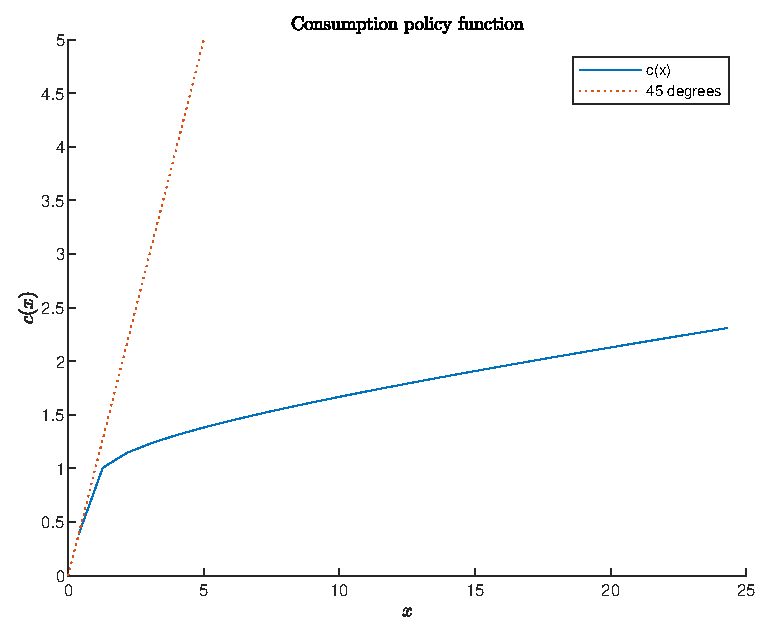
\includegraphics[width=0.7\linewidth]{fig4}
		\label{fig:fig4}
	\end{figure}

Note that for low $x$, the borrowing constraint $x'\geq y$ is binding.
\end{enumerate}
	
\section*{Code}
\subsection*{main.m}
\lstinputlisting[language=Matlab]{"main.m"}
\subsection*{tauchen.m}
\lstinputlisting[language=Matlab]{"tauchen.m"}
\subsection*{rouwenhorst.m}
\lstinputlisting[language=Matlab]{"rouwenhorst.m"}
\subsection*{transition.m}
\lstinputlisting[language=Matlab]{"transition.m"}
\subsection*{policy\_ip.m}
\lstinputlisting[language=Matlab]{"policy_ip.m"}
\subsection*{solve\_ip.m}
\lstinputlisting[language=Matlab]{"solve_ip.m"}
\subsection*{euler\_ip.m}
\lstinputlisting[language=Matlab]{"euler_ip.m"}
\subsection*{policy\_ca.m}
\lstinputlisting[language=Matlab]{"policy_ca.m"}
\subsection*{solve\_ca.m}
\lstinputlisting[language=Matlab]{"solve_ca.m"}
\subsection*{euler\_ca.m}
\lstinputlisting[language=Matlab]{"euler_ca.m"}
\subsection*{markovchain.m}
\lstinputlisting[language=Matlab]{"markovchain.m"}
\subsection*{markovprob.m}
\lstinputlisting[language=Matlab]{"markovprob.m"}

\end{document}
